\section{Detalhes do processo}\label{5-estudo-de-caso-processo-detalhado}

A seguir são listados os passos que compuseram o processo de anotação semântica de forma colaborativo apresentado por este estudo de caso.

\subsection{Passo 1 - Compartilhamento do Projeto}\label{estudo-de-caso-passo1-ambiente-de-trabalho-compartilhado}

O primeiro usuário, denominado \texttt{Usuário A}, já encontrava-se cadastrado na ferramenta e identificado pelo nome de usuário \texttt{mlcalache@gmail.com}. Este usuário foi responsável por carregar a especificação WSDL e a ontologia OWL na ferramenta. O \texttt{Usuário A} também foi responsável por compartilhar o projeto, i.e., a especificação WSDL e a ontologia OWL, com um segundo usuário por meio do \textit{e-mail} \texttt{usuariograsews@gmail.com}. Este segundo usuário, denominado \texttt{Usuário B}, ainda não estava cadastrado na ferramenta. O \texttt{Usuário B} recebeu um \textit{e-mail} com um convite para o trabalho colaborativo. A \figurename~\ref{fig:estudo-de-caso-compartilhar-com-email} ilustra a tela de Grasews informar o \textit{e-mail} do usuário com o qual ele deseja convidar para a edição colaborativa. Já a \figurename~\ref{fig:estudo-de-caso-email-convite} ilustra o \textit{e-mail} recebido pelo \texttt{Usuário B}.

%\begin{landscape}
    \begin{figure}[h]
        %\resizebox{\textwidth}{!}{
            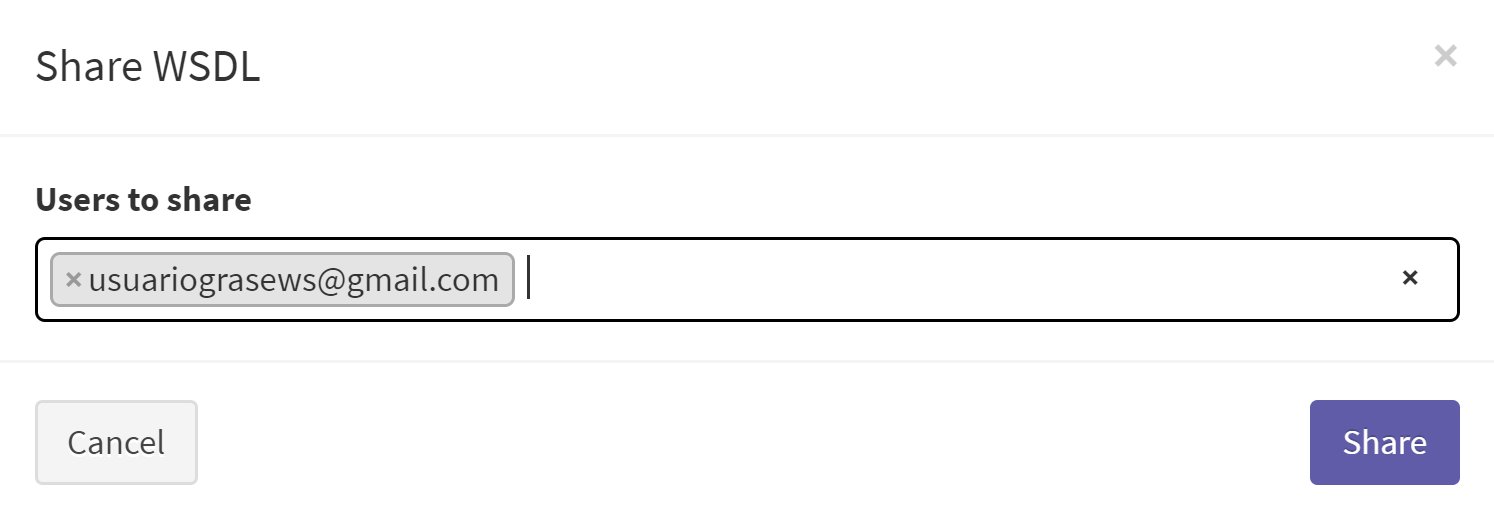
\includegraphics[scale=0.7]{5-grasews-estudo-de-caso/imagens/estudo-de-caso-compartilhar-com-email.png}
        %}
        \centering
        \caption[Compartilhamento do projeto com um outro usuário]{\textbf{Compartilhamento do projeto com um outro usuário.}}
        \label{fig:estudo-de-caso-compartilhar-com-email}
    \end{figure}
%\end{landscape}

%\begin{landscape}
    \begin{figure}[h]
        %\resizebox{\textwidth}{!}{
            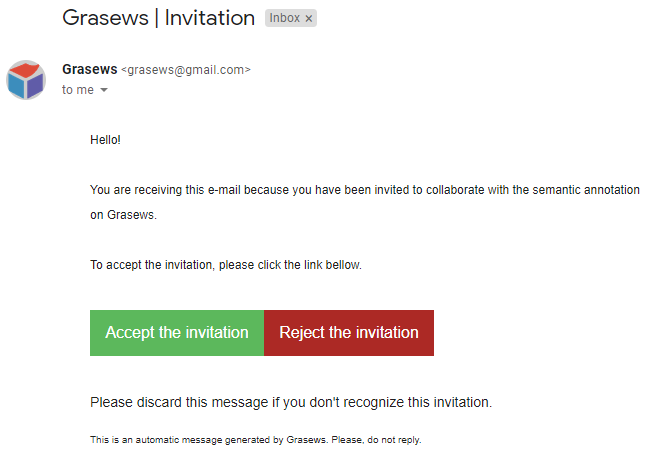
\includegraphics[scale=1.5]{5-grasews-estudo-de-caso/imagens/estudo-de-caso-email-convite.png}
        %}
        \centering
        \caption[\textit{E-mail} de convite para um usuário para o trabalho colaborativo]{\textbf{\textit{E-mail} de convite para um usuário para o trabalho colaborativo.}}
        \label{fig:estudo-de-caso-email-convite}
    \end{figure}
%\end{landscape}

O \texttt{Usuário B}, portanto, teve que se cadastrar na ferramenta. A \figurename~\ref{fig:estudo-de-caso-criar-novo-usuario-por-convite} ilustra a tela de cadastro de um novo usuário por meio de um convite de colaboração.

%\begin{landscape}
    \begin{figure}[h]
        %\resizebox{\textwidth}{!}{
            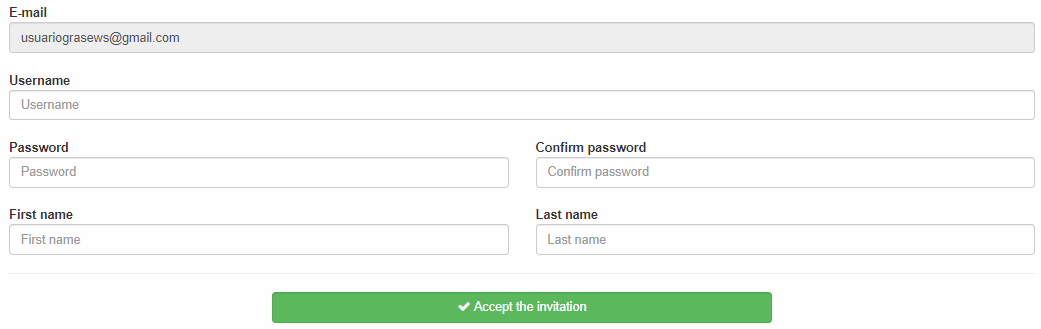
\includegraphics[scale=1.5]{5-grasews-estudo-de-caso/imagens/estudo-de-caso-criar-novo-usuario-por-convite.png}
        %}
        \centering
        \caption[Tela de cadastro de um novo usuário por meio de um convite de colaboração]{\textbf{Tela de cadastro de um novo usuário por meio de um convite de colaboração.}}
        \label{fig:estudo-de-caso-criar-novo-usuario-por-convite}
    \end{figure}
%\end{landscape}

Após ter-se cadastrado e autenticado na ferramenta, o \texttt{Usuário B} pode abrir a mesma especificação WSDL compartilhada pelo \texttt{Usuário A}. A \figurename~\ref{fig:estudo-de-caso-wsdl-compartilhado-disponivel-para-usuario} ilustra a especificação \texttt{MovieStoreServiceSimplified2.0} disponível para o \texttt{Usuário B}.

%\begin{landscape}
    \begin{figure}[h]
        %\resizebox{\textwidth}{!}{
            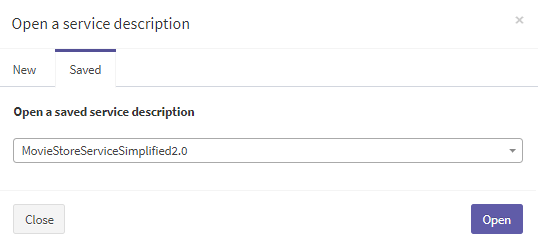
\includegraphics[scale=1.5]{5-grasews-estudo-de-caso/imagens/estudo-de-caso-wsdl-compartilhado-disponivel-para-usuario.png}
        %}
        \centering
        \caption[Especificação WSDL disponível para o \texttt{Usuário B}]{\textbf{Especificação WSDL disponível para o \texttt{Usuário B}.}}
        \label{fig:estudo-de-caso-wsdl-compartilhado-disponivel-para-usuario}
    \end{figure}
%\end{landscape}

\subsection{Passo 2 - Questões}\label{estudo-de-caso-passo2-questoes}

Após os dois usuários terem acesso à mesma especificação WSDL de forma compartilhada, um conjunto de questões relacionadas a elementos da especificação WSDL foram criadas pelos dois usuários.

%A \figurename~\ref{fig:estudo-de-caso-criar-questao} ilustra a tela de Grasews durante a criação de uma questão pelo \texttt{Usuário A}. Neste exemplo, o \texttt{Usuário A} criou uma questão para o elemento tipo complexo XSD \texttt{Genre}. O título de sua questão foi \textit{"Genre meaning"} e a questão em si foi \textit{"What genre stands for?"}.

%%\begin{landscape}
%    \begin{figure}[h]
%        %\resizebox{\textwidth}{!}{
%            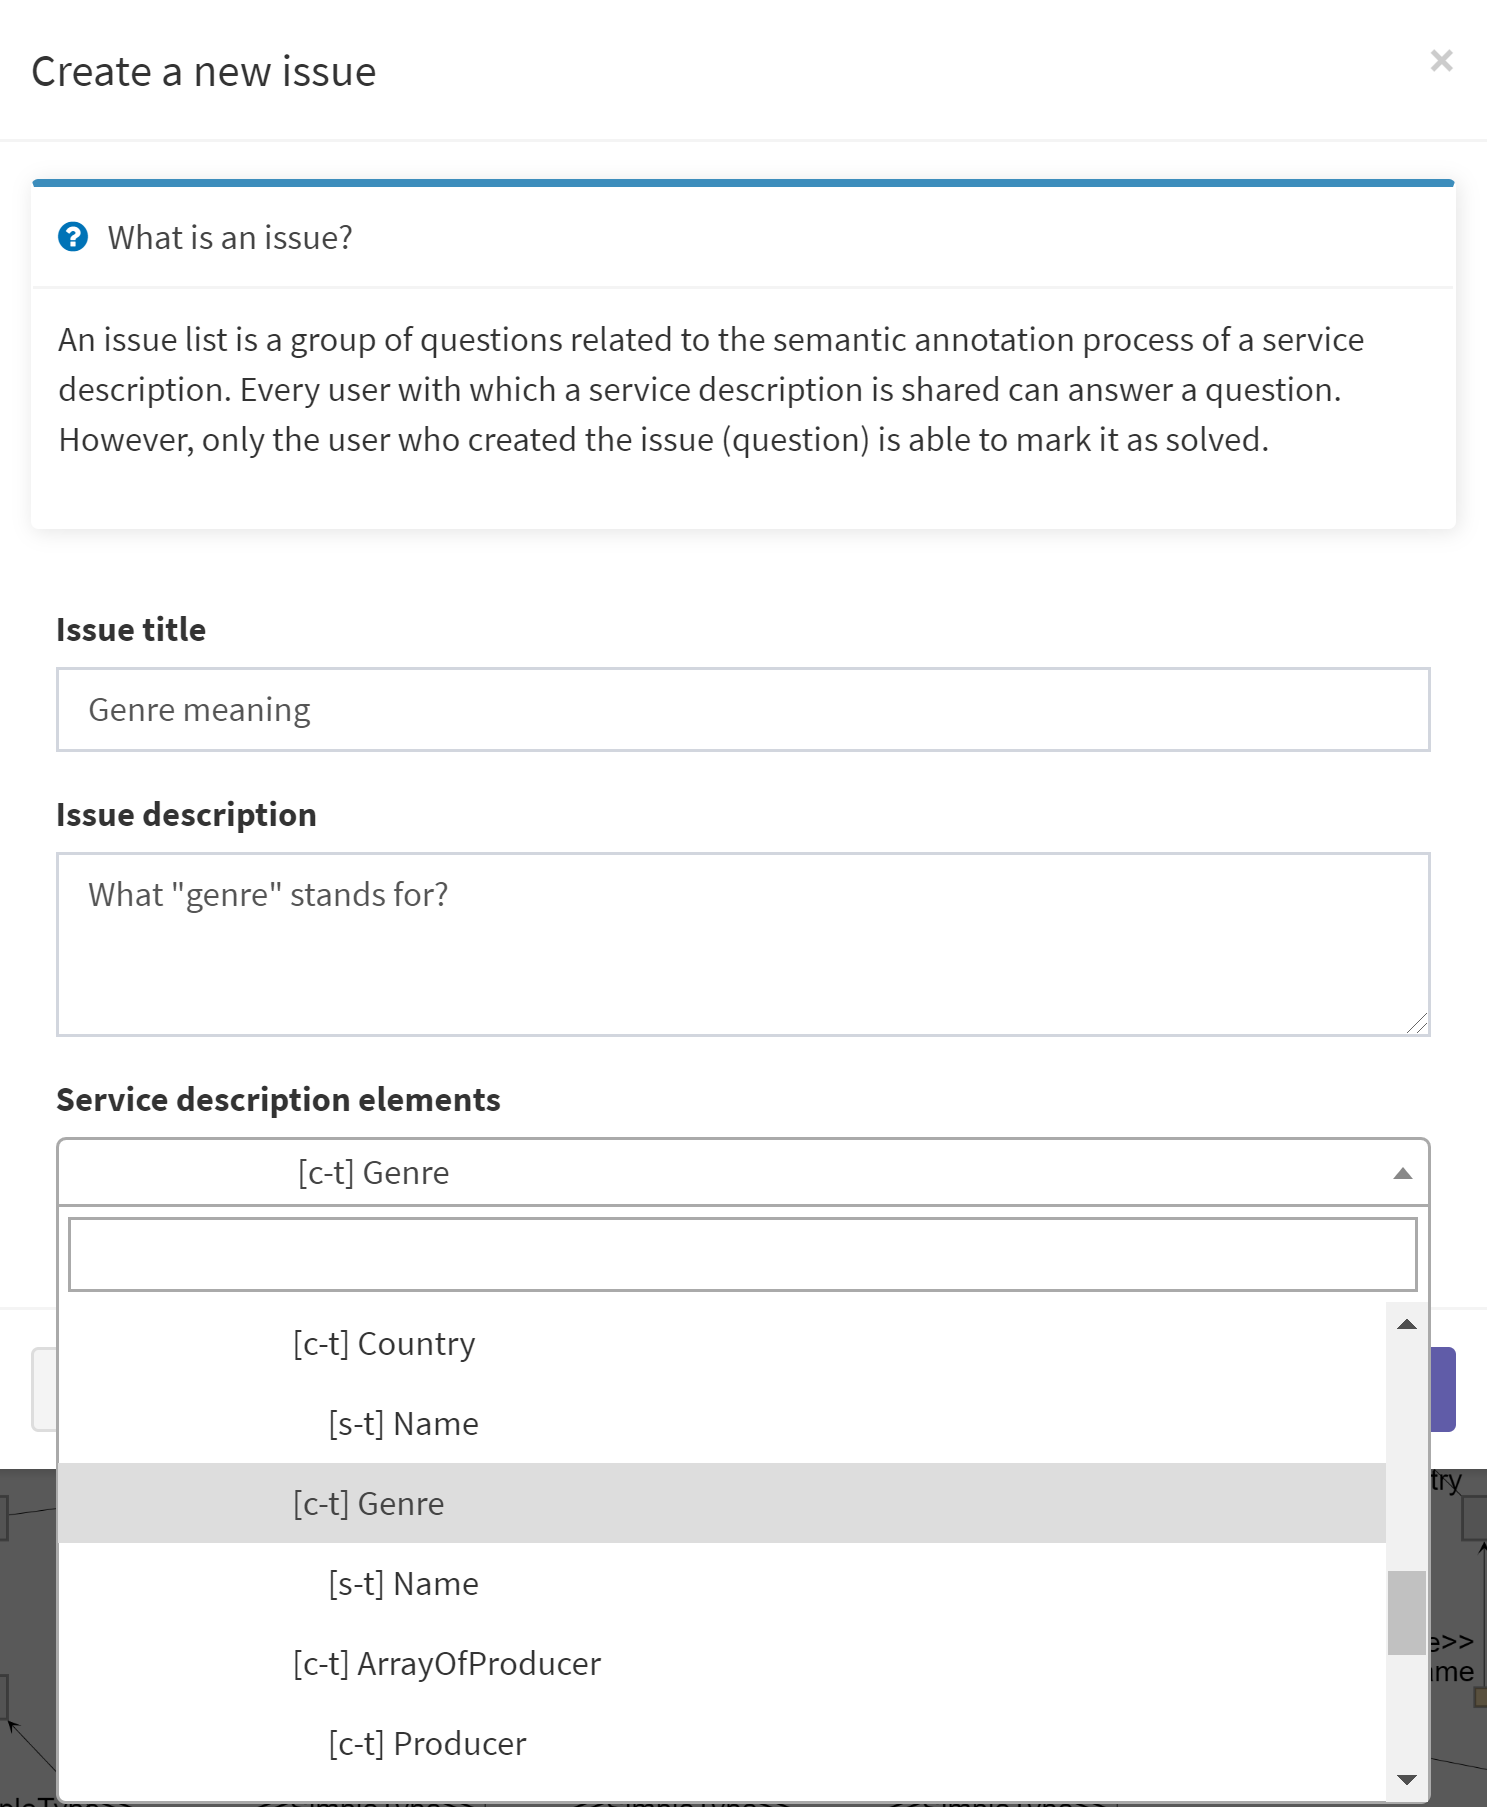
\includegraphics[scale=0.6]{5-grasews-estudo-de-caso/imagens/estudo-de-caso-criar-questao.png}
%        %}
%        \centering
%        \caption[Tela de criação de uma questão pelo \texttt{Usuário A}]{\textbf{Tela de criação de uma questão pelo \texttt{Usuário A}.}}
%        \label{fig:estudo-de-caso-criar-questao}
%    \end{figure}
%%\end{landscape}

Logo que uma nova questão era criada por um usuário, o outro usuário recebia notificações acerca da nova questão. Adicionalmente, o grafo foi automaticamente atualizado a cada questão criada, contendo, portanto, a representação visual para os elementos WSDL/XSD com questões questões associadas. A \figurename~\ref{fig:estudo-de-caso-grafo-wsdl-com-questao} ilustra o elemento tipo complexo XSD \texttt{Genre} com a notação visual para um elemento WSDL/XSD com uma questão, disponível para ambos os usuários. 

%\begin{landscape}
    \begin{figure}[h]
        %\resizebox{\textwidth}{!}{
            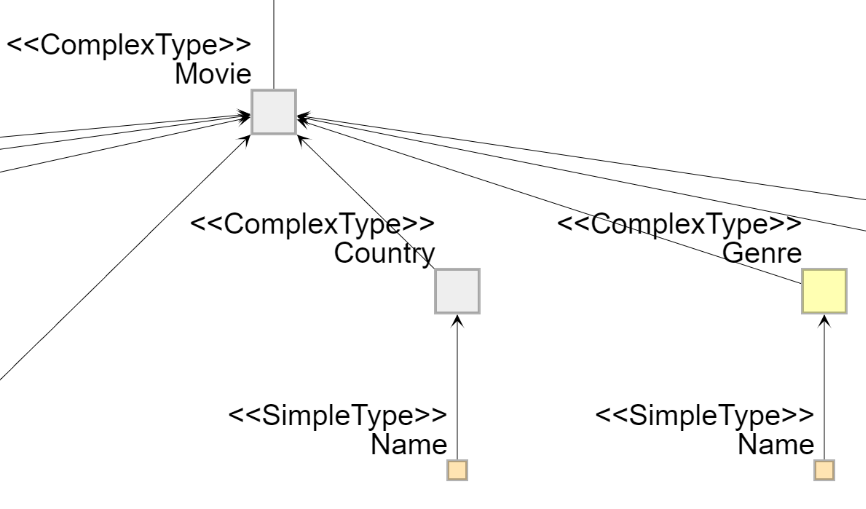
\includegraphics[scale=1]{5-grasews-estudo-de-caso/imagens/estudo-de-caso-grafo-wsdl-com-questao.png}
        %}
        \centering
        \caption[Notação visual para o elemento tipo complexo XSD \texttt{Genre} com uma questão]{\textbf{Notação visual para o elemento tipo complexo XSD \texttt{Genre} com uma questão.}}
        \label{fig:estudo-de-caso-grafo-wsdl-com-questao}
    \end{figure}
%\end{landscape}

De forma assíncrona à criação das questões, ambos usuários adicionaram respostas a elas. O \texttt{Usuário A} adicionou pelo menos uma resposta para cada questão criada pelo \texttt{Usuário A}, enquanto que o \texttt{Usuário B} adicionou pelo menos uma resposta para cada questão criada pelo \texttt{Usuário A}.

Ao passo que as anotações foram feitas e validadas com o auxílio da lista de questões, estas foram marcadas como resolvidas. Ao fim do processo, todas as questões foram marcadas como resolvidas. A seguir são listadas as questões criadas durante o processo.

\begin{tcolorbox}
    \begin{enumerate}[label=(Q\arabic*)]
    %\begin{enumerate}[label={\arabic*}]
        
        % Configura um espaço maior entre parágrafos das questões
        \setlength{\parskip}{0.55cm}
    
		%%%%%%%%%%%%%%%%%%%%%%%%%%%%%%%%%%%%%%%%%%%%%%%%
		
        \item 
        \textbf{Título}: Array of Awards?
        \\
        \textbf{Questão}: Does it mean it is possible to have multiple awards for a single movie?
        \\
        \textbf{Elemento WSDL/XSD}: [c-t] ArrayOfAward
        \\
        \textbf{Usuário}: mlcalache@gmail.com
        \\
        \textbf{Respostas}:
        \begin{enumerate}
            \item
                \textbf{Usuário}: \textit{usuariograsews@gmail.com}
                \\
                \textbf{Resposta}: \textit{Yes. A movie can have multiple awards, such as Oscar and Golden Globe awards.}
        \end{enumerate}
        
        %%%%%%%%%%%%%%%%%%%%%%%%%%%%%%%%%%%%%%%%%%%%%%%%
        
        \item 
        \textbf{Título}: Genre meaning?
        \\
        \textbf{Questão}: What genre stands for?
        \\
        \textbf{Elemento WSDL/XSD}: [c-t] Genre
        \\
        \textbf{Usuário}: mlcalache@gmail.com
        \\
        \textbf{Respostas}:
        \begin{enumerate}
            \item
                \textbf{Usuário}: \textit{usuariograsews@gmail.com}
                \\
                \textbf{Resposta}: \textit{This is the movie category, such as Drama, Comedy, SciFi, etc.}
        \end{enumerate}

        %%%%%%%%%%%%%%%%%%%%%%%%%%%%%%%%%%%%%%%%%%%%%%%%
        
        \item 
        \textbf{Título}: Annotate the complex type of the simple type?
        \\
        \textbf{Questão}: Shoud I annotate the country complex type or the country name simple type?
        \\
        \textbf{Elemento WSDL/XSD}: [c-t] Country
        \\
        \textbf{Usuário}: usuariograsews@gmail.com
        \\
        \textbf{Respostas}:
        \begin{enumerate}
            \item
                \textbf{Usuário}: \textit{mlcalache@gmail.com}
                \\
                \textbf{Resposta}: \textit{Let's focus on the complex types.}
        \end{enumerate}
        
		%%%%%%%%%%%%%%%%%%%%%%%%%%%%%%%%%%%%%%%%%%%%%%%%
        
    % Reconfigura o espaço entre parágrafos
    \setlength{\parskip}{0.2cm}
        
    \end{enumerate}
\end{tcolorbox}

\begin{tcolorbox}
    
    \begin{enumerate}[label=(Q\arabic*)]
        
        % Configura um espaço maior entre parágrafos das questões
        \setlength{\parskip}{0.55cm}
        
        \setcounter{enumi}{3}
        
        %%%%%%%%%%%%%%%%%%%%%%%%%%%%%%%%%%%%%%%%%%%%%%%%
        
        \item 
        \textbf{Título}: Year of movie?
        \\
        \textbf{Questão}: Is there any problem if we don’t have an ontology term for the year of the movie? And what about other elements which we also don’t have an ontology term?
        \\
        \textbf{Elemento WSDL/XSD}: [s-t] Year
        \\
        \textbf{Usuário}: usuariograsews@gmail.com
        \\
        \textbf{Respostas}:
        \begin{enumerate}
            \item
                \textbf{Usuário}: \textit{mlcalache@gmail.com}
                \\
                \textbf{Resposta}: \textit{Let's skip the simple types for now. Let's focus on the complex types. I've created a list of tasks, which does not contemplate the simple types.}
        \end{enumerate}
        
        %%%%%%%%%%%%%%%%%%%%%%%%%%%%%%%%%%%%%%%%%%%%%%%%
        
        \item 
        \textbf{Título}: Actor name?
        \\
        \textbf{Questão}: Since we don’t have a distinct ontology term for the first name and the last name, I suggest we annotate only the Actor element and leave the first and the last name with no annotation. What do you think?
        \\
        \textbf{Elemento WSDL/XSD}: [s-t] FirstName
        \\
        \textbf{Usuário}: usuariograsews@gmail.com
        \\
        \textbf{Respostas}:
        \begin{enumerate}
            \item
                \textbf{Usuário}: \textit{mlcalache@gmail.com}
                \\
                \textbf{Resposta}: \textit{Let's skip the simple types for now. Let's focus on the complex types. I've created a list of tasks, which does not contemplate the simple types.}
        \end{enumerate}
        
		%%%%%%%%%%%%%%%%%%%%%%%%%%%%%%%%%%%%%%%%%%%%%%%%
        
    % Reconfigura o espaço entre parágrafos
    \setlength{\parskip}{0.2cm}
        
    \end{enumerate}
\end{tcolorbox}

%A \figurename~\ref{fig:estudo-de-caso-lista-questoes-nao-resolvidas} ilustra a lista de questões criadas pelos usuários. Note que, pelo ícone e a cor vermelha, não há respostas ainda adicionadas às questões e as questões ainda não estão marcadas como resolvidas.

%%\begin{landscape}
%    \begin{figure}[h]
%        %\resizebox{\textwidth}{!}{
%            \includegraphics[scale=0.8]{5-grasews-estudo-de-caso/imagens/estudo-de-caso-lista-questoes-nao-resol%vidas.png}
%        %}
%        \centering
%        \caption[Lista de questões criadas para a prova de conceito na ferramenta Grasews]{\textbf{Lista de %questões criadas para a prova de conceito na ferramenta Grasews.}}
%        \label{fig:estudo-de-caso-lista-questoes-nao-resolvidas}
%    \end{figure}
%%\end{landscape}

\subsection{Passo 3 - Tarefas}\label{estudo-de-caso-passo3-tarefas}

Simultaneamente com a criação e a resolução das questões, o \texttt{Usuário A} criou uma lista de tarefas que foi compartilhada com o \texttt{Usuário B}. Devido à utilização de conceitos de fácil entendimento do domínio cinematográfico, algumas anotações semânticas podem ser consideradas bastante simples. Neste sentido, o \texttt{Usuário A} foi capaz de realizar anotações semânticas, seguindo a lista de tarefas. O \texttt{Usuário B} contribuiu efetivamente no processo tanto para as iniciadas pelo \texttt{Usuário A}, onde \texttt{Usuário B} pode revisar e corrigir, quanto para as tarefas pendentes, onde \texttt{Usuário B} pode criar as anotações semânticas.

Ao passo que as anotações foram feitas e validadas com o auxílio de tarefas, estas foram marcadas como finalizadas. Ao fim do processo, todas as tarefas foram marcadas como finalizadas. A seguir, são listadas as tarefas criadas durante o processo. 

%Por fim, a \tablename~\ref{tab:estudo-de-caso-lista-questoes} lista as tarefas criadas durante o processo. \hl{fazer}

\begin{tcolorbox}
    \begin{enumerate}[label=(T\arabic*)]
    %\begin{enumerate}[label={\arabic*}]
        
        % Configura um espaço maior entre parágrafos das questões
        \setlength{\parskip}{0.55cm}
        
		%%%%%%%%%%%%%%%%%%%%%%%%%%%%%%%%%%%%%%%%%%%%%%%%
    
        \item 
        \textbf{Título}: Annotate Award Complex Type
        \\
        \textbf{Tarefa}: Annotate Award Complex Type with a Model Reference
        
		%%%%%%%%%%%%%%%%%%%%%%%%%%%%%%%%%%%%%%%%%%%%%%%%
    
        \item 
        \textbf{Título}: Annotate Actor Complex Type
        \\
        \textbf{Tarefa}: Annotate Actor Complex Type with a Model Reference
        
		%%%%%%%%%%%%%%%%%%%%%%%%%%%%%%%%%%%%%%%%%%%%%%%%
    
        \item 
        \textbf{Título}: Annotate Producer Complex Type
        \\
        \textbf{Tarefa}: Annotate Producer Complex Type with a Model Reference
        
		%%%%%%%%%%%%%%%%%%%%%%%%%%%%%%%%%%%%%%%%%%%%%%%%
        
%    % Reconfigura o espaço entre parágrafos
%    \setlength{\parskip}{0.2cm}
%    
%    \end{enumerate}
%\end{tcolorbox}
%
%\begin{tcolorbox}
%    \begin{enumerate}[label=(T\arabic*)]
%    %\begin{enumerate}[label={\arabic*}]
%        
%        % Configura um espaço maior entre parágrafos das questões
%        \setlength{\parskip}{0.55cm}
%        
%        \setcounter{enumi}{3}
        
		%%%%%%%%%%%%%%%%%%%%%%%%%%%%%%%%%%%%%%%%%%%%%%%%
    
        \item 
        \textbf{Título}: Annotate Director Complex Type
        \\
        \textbf{Tarefa}: Annotate Director Complex Type with a Model Reference
        
		%%%%%%%%%%%%%%%%%%%%%%%%%%%%%%%%%%%%%%%%%%%%%%%%
		
        \item 
        \textbf{Título}: Annotate Country Complex Type
        \\
        \textbf{Tarefa}: Annotate Country Complex Type with a Model Reference
        
		%%%%%%%%%%%%%%%%%%%%%%%%%%%%%%%%%%%%%%%%%%%%%%%%
		
        \item 
        \textbf{Título}: Annotate Genre Complex Type
        \\
        \textbf{Tarefa}: Annotate Genre Complex Type with a Model Reference
        
		%%%%%%%%%%%%%%%%%%%%%%%%%%%%%%%%%%%%%%%%%%%%%%%%
		
        \item 
        \textbf{Título}: Annotate Movie Complex Type
        \\
        \textbf{Tarefa}: Annotate Movie Complex Type with a Model Reference
        
		%%%%%%%%%%%%%%%%%%%%%%%%%%%%%%%%%%%%%%%%%%%%%%%%
        
    % Reconfigura o espaço entre parágrafos
    \setlength{\parskip}{0.2cm}
    
    \end{enumerate}
\end{tcolorbox}

%A \figurename~\ref{fig:estudo-de-caso-lista-tarefas} ilustra a interface gráfica de Grasews para a lista de tarefas criadas pelo \texttt{Usuário A}.

%Note que, pelo ícone e a cor vermelha, não há comentários ainda adicionados às tarefas e as tarefas ainda não estão marcadas como finalizadas.

%%\begin{landscape}
%    \begin{figure}[h]
%        %\resizebox{\textwidth}{!}{
%            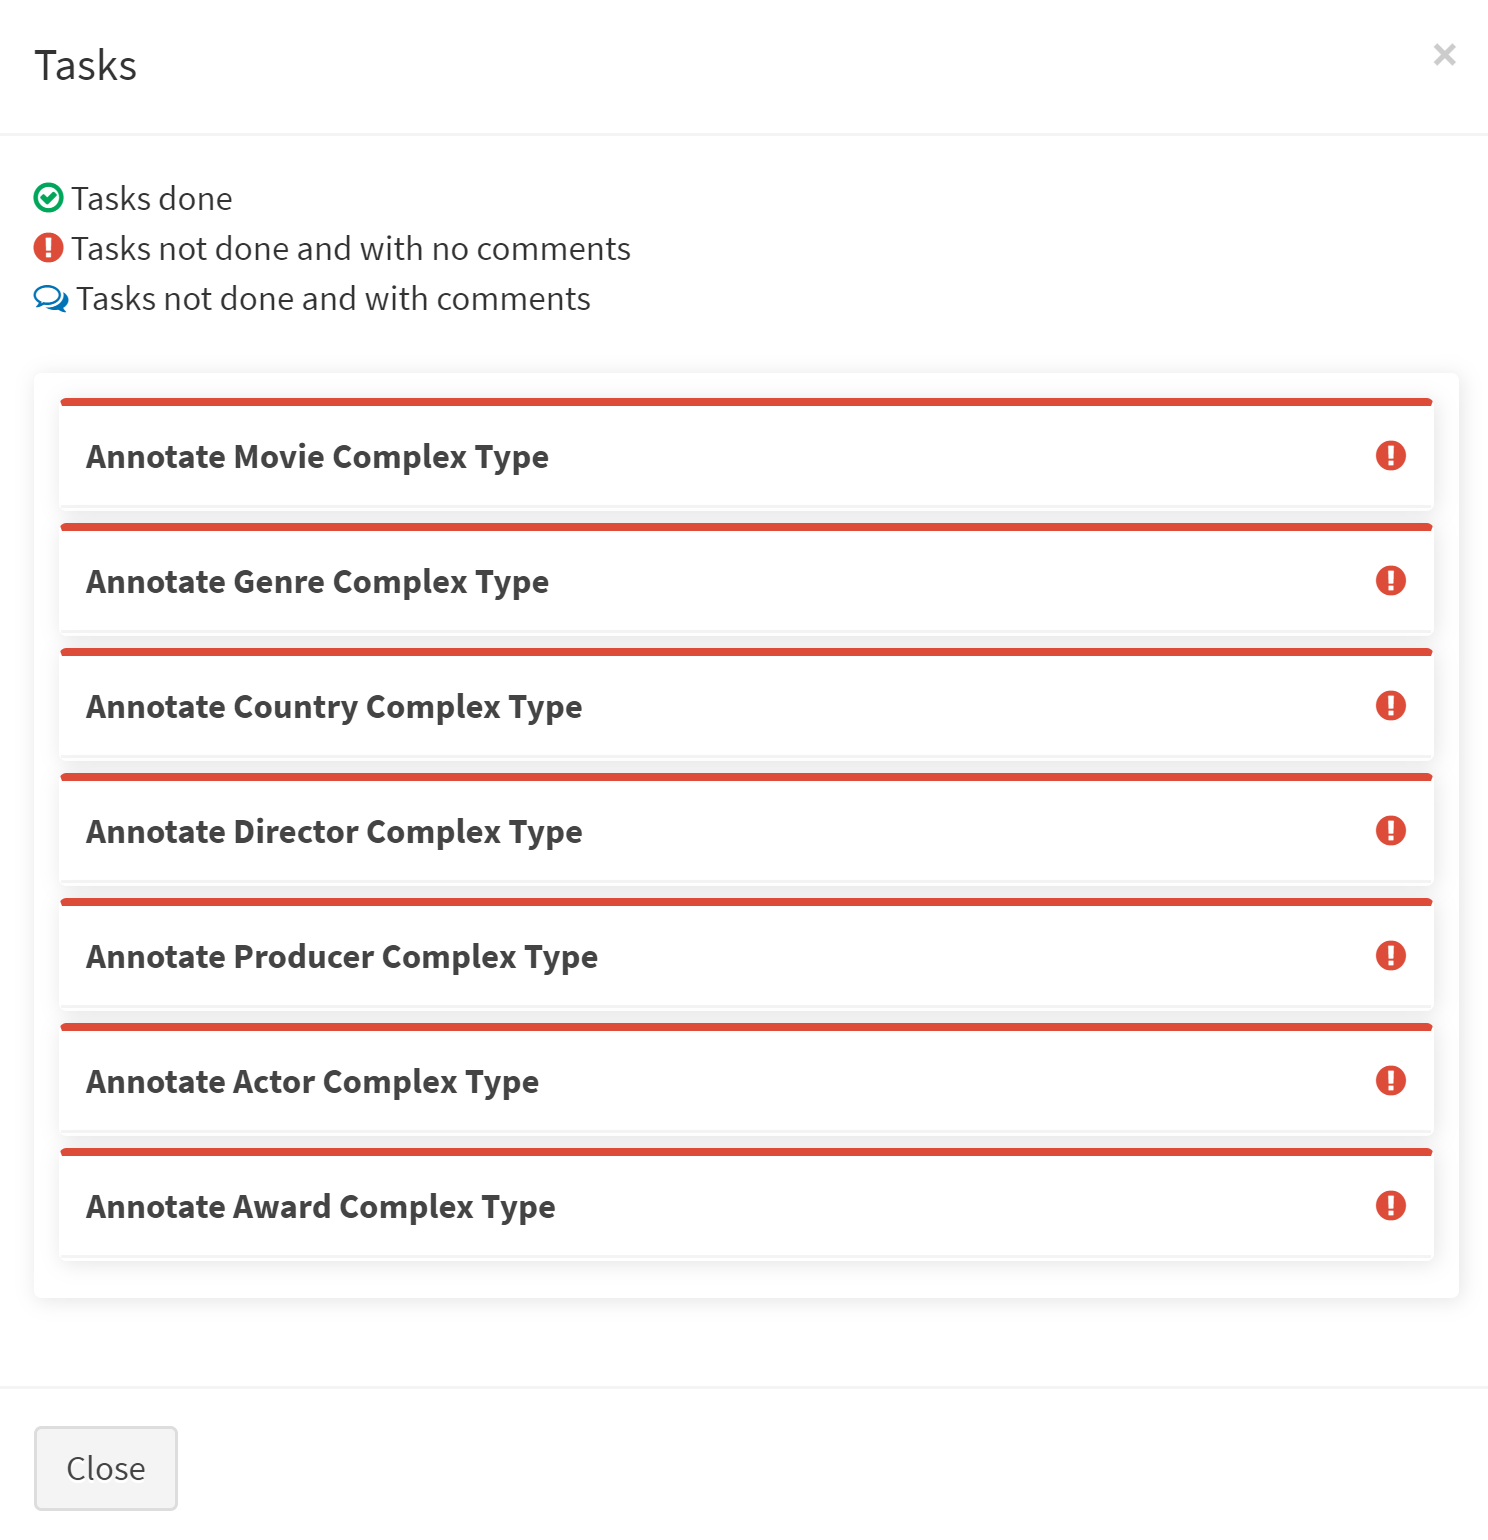
\includegraphics[scale=0.8]{5-grasews-estudo-de-caso/imagens/estudo-de-caso-lista-tarefas.png}
%        %}
%        \centering
%        \caption[Lista de tarefas criadas para a prova de conceito na ferramenta Grasews]{\textbf{Lista de %tarefas criadas para a prova de conceito na ferramenta Grasews.}}
%        \label{fig:estudo-de-caso-lista-tarefas}
%    \end{figure}
%%\end{landscape}

\iffalse
\begin{landscape}
    \begin{table}[ht!]
        \setlength{\tabcolsep}{10pt} % Default value: 6pt
        \renewcommand{\arraystretch}{1.5} % Default value: 1
        \centering
    	\caption[Lista de questões criadas durante o processo.]{\textbf{Lista de questões criadas durante o processo.}}
    	\label{tab:estudo-de-caso-lista-questoes}
    	%\resizebox{\textwidth}{!}{
    		\begin{tabular}{| >{\columncolor{Gray}}c | c | c | c | c | }
    			\hline
                \rowcolor{Gray}
    			
    			{\textbf{\#}} & \textbf{Título} & \textbf{Questão} & \textbf{Elemento WSDL/XSD} & \textbf{Usuário}
    			
    			%%%%%%%%%%%%%%%%%%%%%%%%%%%%%%%%%%%%%%%%%%%%%%%%
    			\\
    			\hline
    			{}
    			& {}
    			& {Does it mean it is}
    			& {}
    			& {}
    			\\
    			{}
    			& {}
    			& {possible to have multiple}
    			& {}
    			& {}
    			\\
    			\multirow{-2.5}{*}[3px]{1}
    			& \multirow{-2.5}{*}[3px]{Array Of Awards?}
    			& {awards for a single movie?}
    			& \multirow{-2.5}{*}[3px]{[c-t] ArrayOfAward}
    			& \multirow{-2.5}{*}[3px]{mlcalache@gmail.com}
    			
    			%%%%%%%%%%%%%%%%%%%%%%%%%%%%%%%%%%%%%%%%%%%%%%%%
    			
    			\\
                \hline
    			{2} & {Genre meaning?} & {What genre stands for?} & {[c-t] Genre} & {mlcalache@gmail.com}
    			
    			%%%%%%%%%%%%%%%%%%%%%%%%%%%%%%%%%%%%%%%%%%%%%%%%
    			
    			\\
    			\hline
    			{}
    			& {Annotate}
    			& {Shoud I annotate the}
    			& {}
    			& {}
    			\\
    			{}
    			& {complex type}
    			& {country complex type or}
    			& {}
    			& {}
    			\\
    			\multirow{-2.5}{*}[3px]{3}
    			& {or simple type?}
    			& {the country name simple type?}
    			& \multirow{-2.5}{*}[3px]{[c-t] Country}
    			& \multirow{-2.5}{*}[3px]{usuariograsews@gmail.com}
    			
    			%%%%%%%%%%%%%%%%%%%%%%%%%%%%%%%%%%%%%%%%%%%%%%%%
    			
    			\\
    			\hline
    			{}
    			& {}
    			& {Is there any problem if wedon't have}
    			& {}
    			& {}
    			\\
    			{}
    			& {}
    			& {an ontology term for the year}
    			& {}
    			& {}
    			\\
    			{}
    			& {}
    			& {of the movie? And what about}
    			& {}
    			& {}
    			\\
    			{}
    			& {}
    			& {other elements which we also}
    			& {}
    			& {}
    			\\
    			\multirow{-4.5}{*}[3px]{4}
    			& \multirow{-4.5}{*}[3px]{Year of movie?}
    			& {don't have an ontology term?}
    			& \multirow{-4.5}{*}[3px]{[s-t] Year}
    			& \multirow{-4.5}{*}[3px]{usuariograsews@gmail.com}
    			
    			%%%%%%%%%%%%%%%%%%%%%%%%%%%%%%%%%%%%%%%%%%%%%%%%
    			
    			\\
    			\hline
    			{}
    			& {}
    			& {Since we don't have a distinct ontology}
    			& {}
    			& {}
    			\\
    			{}
    			& {}
    			& {term for the first name and the last name,}
    			& {}
    			& {}
    			\\
    			{}
    			& {}
    			& {I suggest we annotate only the Actor element}
    			& {}
    			& {}
    			\\
    			{}
    			& {}
    			& {and leave the first and the last name}
    			& {}
    			& {}
    			\\
    			\multirow{-4.5}{*}[3px]{5}
    			& \multirow{-4.5}{*}[3px]{Actor name?}
    			& {with no annotation. What do you think?}
    			& \multirow{-4.5}{*}[3px]{[s-t] FirstName}
    			& \multirow{-4.5}{*}[3px]{usuariograsews@gmail.com}
    			
    			%%%%%%%%%%%%%%%%%%%%%%%%%%%%%%%%%%%%%%%%%%%%%%%%
    			
    			\\
                \hline
    		\end{tabular}
    	%}
    \end{table}
\end{landscape}
\fi

\iffalse
\begin{table}[ht!]
    \setlength{\tabcolsep}{10pt} % Default value: 6pt
    \renewcommand{\arraystretch}{1.5} % Default value: 1
    \centering
	\caption[Lista de tarefas criadas durante o processo.]{\textbf{Lista de tarefas criadas durante o processo.}}
	\label{tab:estudo-de-caso-lista-questoes}
	%\resizebox{\textwidth}{!}{
		\begin{tabular}{| >{\columncolor{Gray}}c | c | c | }
			\hline
            \rowcolor{Gray}
			{\#} & \textbf{Tarefa}
			\\
			\hline
			{1} & {bla bla bla}
			\\
            \hline
			{2} & {bla bla bla}
			\\ 
            \hline
			{3} & {bla bla bla}
			\\
            \hline
		\end{tabular}
	%}
\end{table}
\fi

\subsection{Passo 4 - Anotação Semântica}\label{estudo-de-caso-passo4-anotacao-semantica}

O último passo da prova de conceito consiste da anotação semântica da especificação WSDL.
Ambos usuários trabalharam simultaneamente na anotação semântica conforme a lista de tarefas criada pelo \texttt{Usuário A}. A anotação semântica foi feita tanto por meio do menu de contexto do grafo, quanto por meio do menu de contexto do menu \textit{tree-view} WSDL e do menu \textit{tree-view} OWL. 

O documento de especificação WSDL anotado encontra-se disponível no endereço \url{https://raw.githubusercontent.com/mlcalache/wsdls/master/MovieStoreServiceSimplified2.0-anotado.wsdl}. Adicionalmente, a especificação WSDL anotada está disponível no Anexo \ref{anexo-WSDL-anotado-estudo-de-caso}. Por fim, a \figurename~\ref{fig:estudo-de-caso-grafo-wsdl-anotado} ilustra o grafo WSDL do \texttt{Usuário B} após a conclusão das tarefas. Como resultado, temos a especificação WSDL anotada 

\begin{landscape}
    \begin{figure}[h]
        %\resizebox{\textwidth}{!}{
            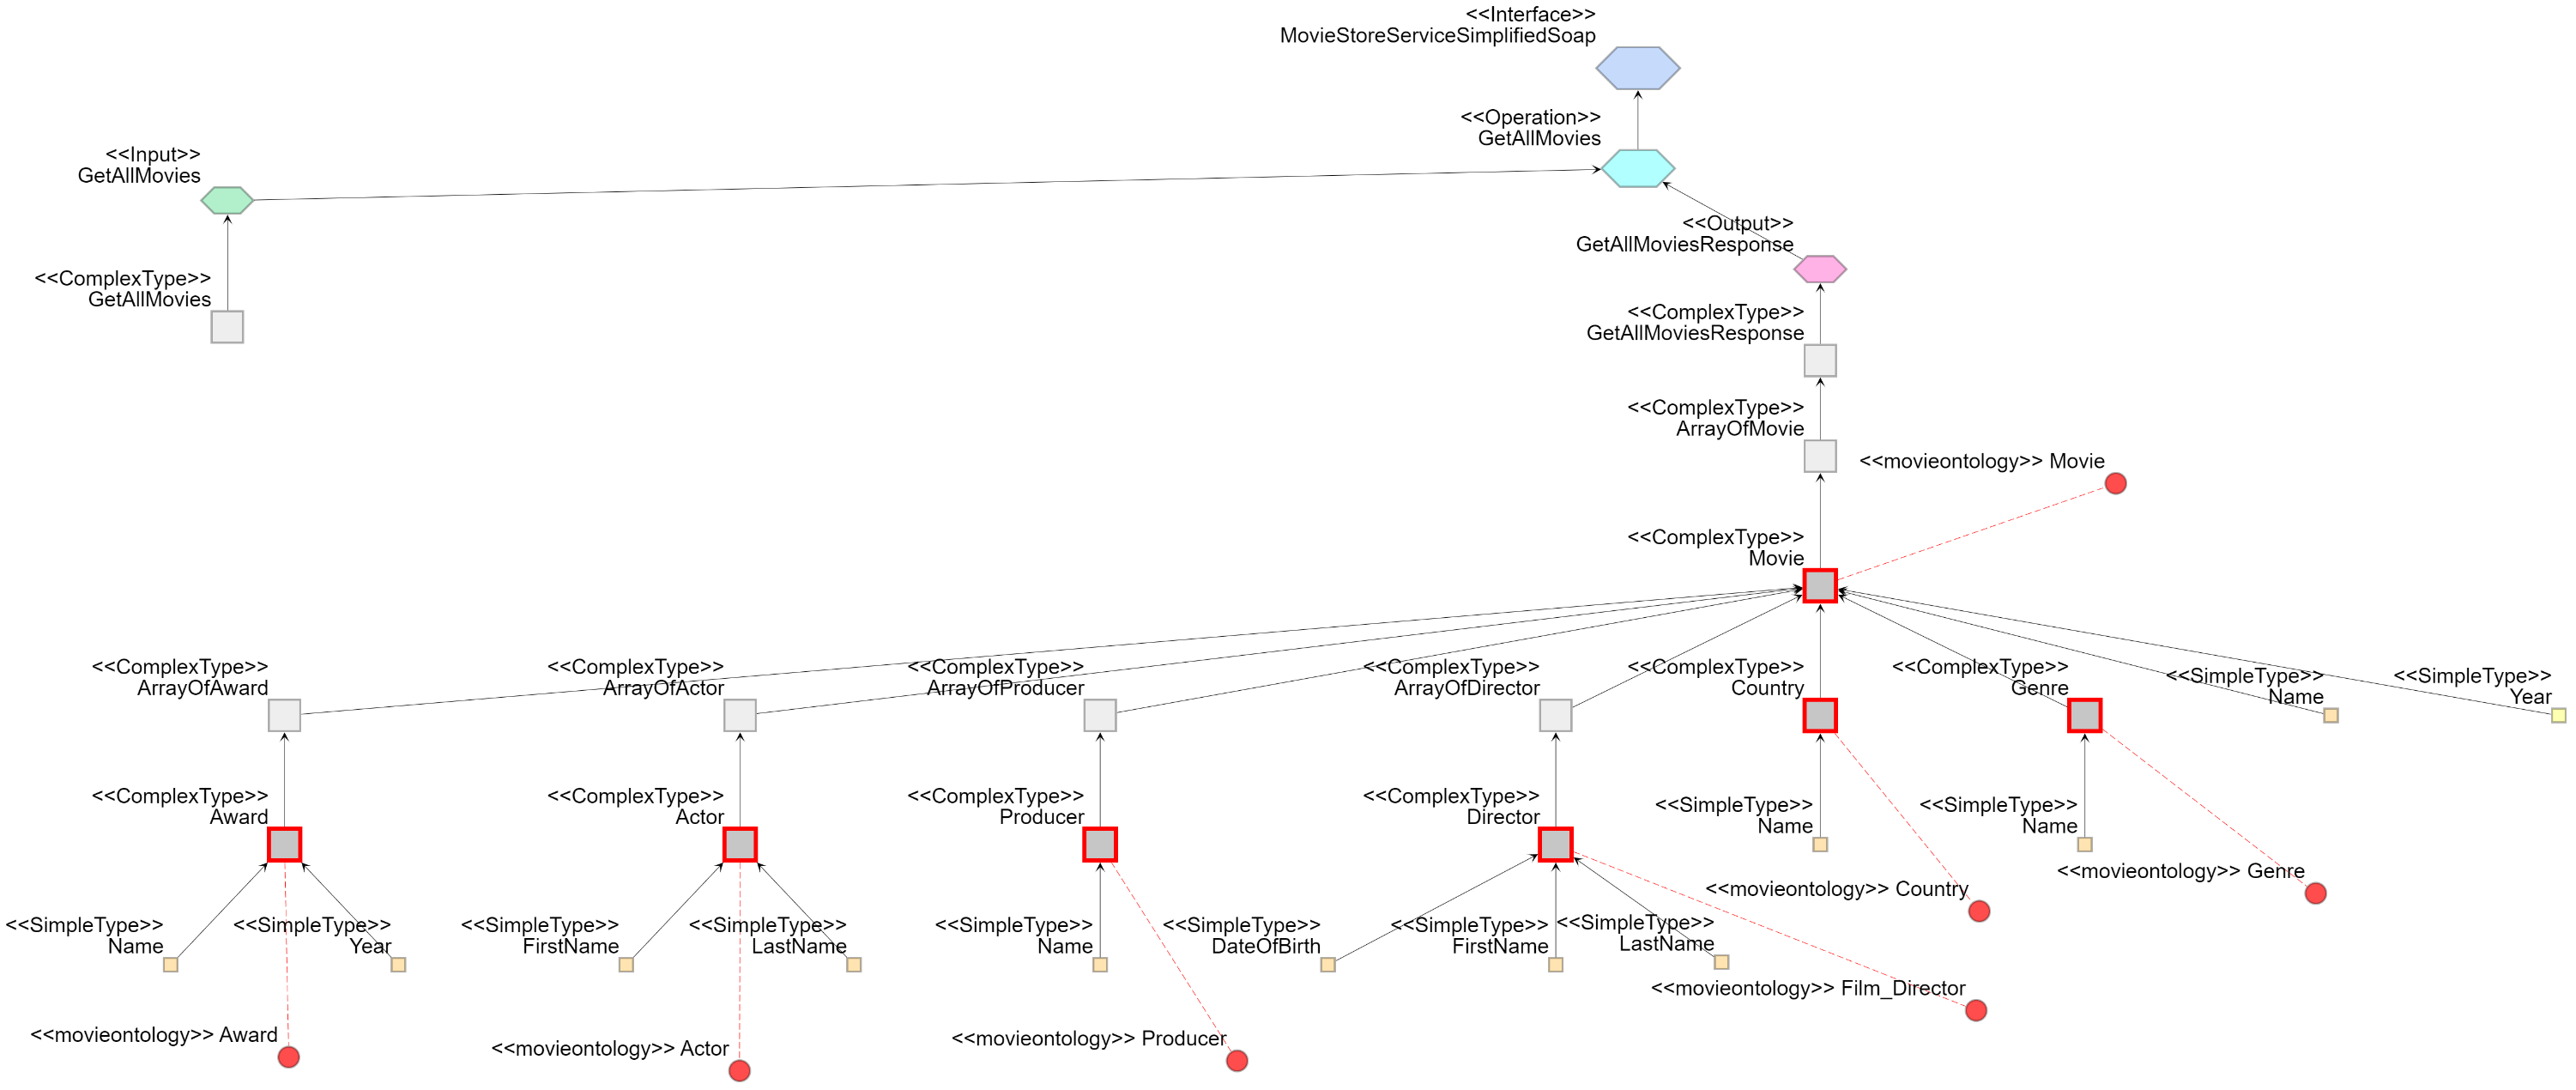
\includegraphics[scale=0.78]{5-grasews-estudo-de-caso/imagens/estudo-de-caso-grafo-wsdl-anotado.png}
        %}
        \centering
        \caption[Grafo da especificação WSDL anotada na prova de conceito]{\textbf{Grafo da especificação WSDL anotada na prova de conceito.}}
        \label{fig:estudo-de-caso-grafo-wsdl-anotado}
    \end{figure}
\end{landscape}